\documentclass[conference]{IEEEtran}
\usepackage[utf8]{inputenc}
\usepackage{amsmath,amssymb,graphicx,booktabs}

\begin{document}

\title{Self-Supervised JEPA Pretraining for ECG Representations with Aligned Clinical Reports}

\author{\IEEEauthorblockN{Dheiver Francisco Santos, PhD}
\IEEEauthorblockA{Independent Researcher\\
Maceió, Alagoas, Brazil\\
ORCID: https://orcid.org/0000-0002-8599-9436}}

\maketitle

\begin{abstract}
Labeled electrocardiograms (ECG) are scarce, while unlabeled recordings are abundant. We pretrain a joint-embedding predictive architecture (JEPA) on unlabeled ECG segments by predicting the embeddings of masked leads and segments, and we align the resulting representations with clinical report text. We evaluate on a public 12-lead benchmark with a linear probe and a low-label regime, and on synthetic ECG with controlled anomalies. This is a research protocol, not a clinical tool. A synthetic pilot is too easy to discriminate, so the pretraining results are pending.
\end{abstract}

\begin{IEEEkeywords}
electrocardiogram, self-supervised learning, JEPA, clinical text alignment, time series
\end{IEEEkeywords}

\section{Introduction}
Supervised ECG models need expert labels that are expensive to obtain. Self-supervised pretraining reduces this cost. We ask whether predicting embeddings of masked ECG segments, rather than reconstructing signals, gives representations that transfer to diagnostic classification with few labels, and whether alignment to clinical report text improves them.

\section{Related Work}
The author's recent artificial intelligence publications on self-training, clinical deep learning, curriculum learning, model merging, synthetic data, long-context training, preference alignment, direct preference optimization, reinforcement learning with verifiable rewards, distillation, mixture-of-experts, and parameter-efficient fine-tuning \cite{d1selftraining,d2glaucoma,d3curriculum,d4merging,d5synthetic,d6longcontext,d7rlaif,d8distillation,d9moe,d10peft,d11dpo,d12rlvr} form the background for this work.

JEPA-style objectives in embedding space are described in \cite{bardes2024vjepa}. Masked reconstruction for signals is a common baseline. The author's recent work on a glaucoma detection study using clinical data \cite{d2glaucoma} and on fine-tuning efficiency \cite{d10peft} motivates the clinical evaluation design and the low-label regime.

\section{Method}
A 12-lead ECG of length $T$ is split into segments. A segment encoder $f_\theta$ produces embeddings; masked segments are predicted by $g_\phi$ from visible context, with the target given by a stop-gradient encoder. A text encoder maps the clinical report to an embedding, and a contrastive alignment term links it to the ECG embedding of the same patient.

\subsection*{Equations and their meaning}
Each segment $x$ is embedded and a masked segment is predicted from visible context. The JEPA loss is
\begin{equation}
\mathcal{L}_{\mathrm{JEPA}}=\big\lVert g_\phi\big(f_\theta(x_{\mathrm{vis}})\big)-\bar f(x_{\mathrm{mask}})\big\rVert_2^2,
\end{equation}
where $x_{\mathrm{vis}}$ are the visible leads or segments, $x_{\mathrm{mask}}$ the hidden ones, and $\bar f$ a stop-gradient target encoder. Alignment with clinical report text $t$ uses a symmetric contrastive (InfoNCE) term over a batch of $B$ ECG--report pairs:
\begin{equation}
\mathcal{L}_{\mathrm{align}}=-\frac{1}{B}\sum_{i=1}^{B}\log\frac{\exp\big(\mathrm{sim}(e_i,t_i)/\tau\big)}{\sum_{j=1}^{B}\exp\big(\mathrm{sim}(e_i,t_j)/\tau\big)},
\end{equation}
where $e_i$ and $t_i$ are the ECG and report embeddings of pair $i$, $\mathrm{sim}$ is cosine similarity, and $\tau$ a temperature. The term pulls matched pairs together and pushes mismatched pairs apart.

The pilot reduces each segment to $16$ principal components, $z=(x-\mu)V_{16}$, where $V_{16}$ holds the top eigenvectors of the unlabeled covariance. The classifier is logistic regression,
\begin{equation}
P(y=1\mid z)=\sigma(w^\top z+b),\qquad \sigma(u)=\frac{1}{1+e^{-u}},
\end{equation}
and performance is the accuracy $\mathrm{Acc}=\frac{1}{N}\sum_n\mathbf{1}[\hat y_n=y_n]$ on held-out beats, with $\hat y_n=\mathbf{1}[P(y_n=1\mid z_n)\ge 0.5]$.

\section{Experimental Protocol}
\textbf{Public benchmark.} A public 12-lead ECG dataset with diagnostic superclasses. Evaluation uses a linear probe, macro-AUROC, and label fractions of 1\%, 10\%, and 100\%.

\textbf{Synthetic ECG.} Waveforms generated from a parametric model with controlled rhythm and morphology anomalies, to test sensitivity to each anomaly type.

\textbf{Report alignment.} Paired reports are used when available; the ablation without alignment is reported.

\textbf{Baselines.} Random initialization, masked reconstruction, and supervised training on the same label fractions.

\textbf{Statistics.} Five seeds, 95\% bootstrap intervals, and a patient-level split to avoid leakage.

\textbf{Ethics.} Only public, de-identified data are used. No clinical use is claimed.

\section{Results}
This pilot arm uses synthetic sinusoidal beats with a two-class frequency change, not the ECG benchmark. A PCA readout (16 components fit on unlabeled data) and a raw-signal logistic regression both reach 0.995 or higher across label fractions from 2\% to 50\%. The task is too easy to show any benefit of pretraining. The JEPA pretraining, the report alignment, and PTB-XL remain pending.

\begin{figure}[!t]
\centering
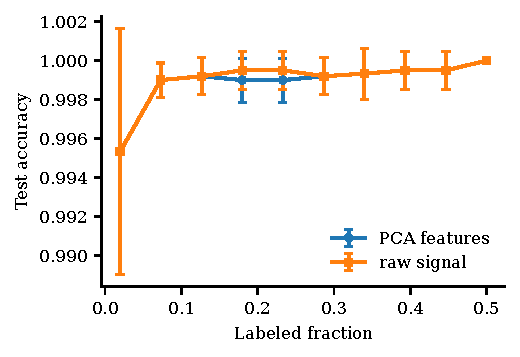
\includegraphics[width=\columnwidth]{figs/fig08_ecg.pdf}
\caption{Test accuracy versus labeled fraction for PCA features and raw signal (synthetic pilot).}
\label{fig:fig08_ecg}
\end{figure}

\section{Discussion and Limitations}
Public benchmarks may not represent the population of the target use. Report-based alignment may learn reporting style rather than physiology, which the ablation addresses.

\section{Conclusion}
We propose JEPA pretraining with report alignment for ECG and a protocol with patient-level splits, low-label regimes, and synthetic anomalies.

\section*{Acknowledgments}
The author thanks the Brazilian artificial intelligence community.

\nocite{ctl_full_names}
\bibliographystyle{IEEEtran}
\bibliography{refs}

\end{document}
